\documentclass[11pt,twoside]{article}
% \input{hwheader.tex}

%\documentclass[11pt,twoside]{article}
\usepackage[nonamelimits]{amsmath}
\usepackage{amssymb, amsthm}

\setlength{\oddsidemargin}{0 in}
\setlength{\evensidemargin}{0 in}
\setlength{\topmargin}{-0.6 in}
\setlength{\textwidth}{6.5 in}
\setlength{\textheight}{8.5 in}
\setlength{\headheight}{0.5 in}
\setlength{\headsep}{0.5 in}
\setlength{\parindent}{0 in}
\setlength{\parskip}{0.1 in}

%%% SETS
\newcommand\Z{\mbox{$\mathbb Z$}}
\newcommand\N{\mbox{$\mathbb N$}}
\newcommand\R{\mbox{$\mathbb R$}}
\newcommand\F{\mbox{$\mathbb F$}}
\def\B{\{0,1\}}
\def\cond{\mid}

%%% FUNCTIONS
\providecommand\floor[1]{\lfloor#1\rfloor}
\providecommand\ceil[1]{\lceil#1\rceil}
\providecommand\blog[1]{\log_2\ceil{#1}}
\providecommand\abs[1]{\lvert#1\rvert}
\providecommand\bigabs[1]{\bigl\lvert#1\bigr\rvert}

\def\co{{\rm co}}
\def\avg{{\rm Avg}}
\def\heur{{\rm Heur}}

%%% THEOREM TYPE ENVIRONMENTS
\newtheorem{theorem}{Theorem}
\newtheorem{lemma}[theorem]{Lemma}
\newtheorem{corollary}[theorem]{Corollary}
\newtheorem{proposition}[theorem]{Proposition}
\newtheorem{claim}[theorem]{Claim}
\newtheorem{exercise}{Exercise}
\newtheorem{conjecture}{Conjecture}
\newtheorem{example}{Example}
\newtheorem{remark}{Remark}
\newtheorem{definition}[theorem]{Definition}

%%% HEADINGS
\newcommand{\homework}[1]{
   \pagestyle{myheadings}
   \thispagestyle{plain}
   \newpage
   \setcounter{page}{1}
   \noindent
   \classname \hfill \mbox{\updatedday} \\
   \instname \hfill \mbox{\duedate}
   \rule{6.5in}{0.5mm}
   \vspace*{-0.1 in}
}


\newcommand{\problem}[1]{\section*{Problem #1}}


\renewcommand{\labelenumi}{(\alph{enumi})}
\renewcommand{\labelenumii}{(\roman{enumii})}

%%% DEFINITIONS
\def\classname{CSCI-SHU 220: Algorithms @ NYU Shanghai}


%%% INSTRUCTIONS
\raggedbottom 


\usepackage[pdftex]{graphicx}
\usepackage{pgf,tikz}
\usetikzlibrary{shapes,arrows,automata}

\usepackage{listings}
\usepackage{xcolor}
\lstset { %
    language=C++,
    backgroundcolor=\color{black!5}, % set backgroundcolor
    basicstyle=\footnotesize,% basic font setting
}

\newcommand\includefa[1]{\begin{center}\includegraphics[scale=0.5]{#1}\end{center}}

\def\updatedday{Posted: April 7, 2024}
\def\duedate{Due: 11:30pm (Shanghai time), April 17, 2024}
\newenvironment{solution}{{\par\noindent\it Solution.}}{}

\def\instname{Homework 3}

\pagenumbering{gobble}

\begin{document}
\homework{1}

This assignment has in total $55$ base points and $10$ extra points, and the cap is $55$.
Bonus questions are indicated using the $\star$ mark.

\textit{Please specify the following information before submission}:
\begin{itemize}
    \item Your Name: Yufeng Xu %  (put your name here)
    \item Your NetID: yx3038 % (put your NetID here)
\end{itemize}

\problem{1: Infinite knapsack [$10^\star+15$ pts]}
Recall that in the infinite knapsack problem, we are given a knapsack with capacity $W$ and $m$ types of (infinite) items $I_1,\dots,I_m$, where $I_i$ has weight $w_i \in \mathbb{N}$ and value $v_i \in \mathbb{R}_{>0}$.
Our goal is to include in the knapsack items of total weight at most $W$ with maximum total value.
Formally, we want to compute $m$ non-negative integers $n_1,\dots,n_m$ satisfying $\sum_{i=1}^m n_i w_i \leq W$ such that $\sum_{i=1}^m n_i v_i$ is maximized (here $n_i$ indicates the number of copies of $I_i$ included in the knapsack).
In the lecture, we have already seen that this problem can be solved in $O(mW)$ time.
In this exercise, we try to design another algorithm with running time $O(mw_{\max}^2)$ where $w_{\max} = \max_{i=1}^m w_i$.
This task is somehow challenging.
So we divide it into the following two steps.
Also, for simplicity, we assume that the value-weight ratios of the items are distinct and sorted, i.e., $\frac{v_1}{w_1} > \frac{v_2}{w_2} > \cdots > \frac{v_m}{w_m}$.

\begin{enumerate}
    \item[(a)$^\star$] Prove that in any optimal solution $(n_1,\dots,n_m)$, the total number of copies of the items $I_2,\dots,I_m$ included in the knapsack is at most $w_{\max}-1$, i.e., $\sum_{i=2}^m n_i \leq w_{\max}-1$.
    \item[(b)] Based on the conclusion of (a), design an algorithm $\textsc{Knapsack}(m,W,(w_1,v_1),\dots,(w_m,v_m))$ for infinite knapsack with running time $O(mw_{\max}^2)$.
    For convenience, your algorithm only need to return the maximum value achieved.
    Describe the basic idea and give the pseudocode.
    Briefly justify the correctness and analyze the time complexity. \\[1ex]
    (\textbf{Hint:} According to (a), we know that, in an optimal solution, the total \textit{weight} of the items $I_2,\dots,I_m$ is $O(w_{\max}^2)$, and hence the item $I_1$ occupies ``most'' space of the knapsack. Try to combine this observation with the $O(mW)$-time DP algorithm.)
\end{enumerate}

\begin{solution}
\textbf{Please write down your solution to Problem 1 here.}
\vspace{10pt}\\
\textbf{(a)} We prove the problem by contradiction. Suppose there exists an optimal solution where $\sum_{i=2}^{m}n_i\geq w_{\text{max}}$.
We denote these items as $w_1',w_2',\dots w_n'$ where $n\geq w_{\text{max}}$, and for each $w_j'$, $\exists i=2,\dots, m$ such that $w_j'=w_i$. 
There can be multiple $w_j'$s that are equal to the same $w_i$.
\vspace{10pt}\\
Now, we want to show that $\exists 1\leq l\leq r\leq n$ such that $\sum_{j=l}^{r}w_j'$ is a multiple of $w_1$.
Consider the sum of the first $k$ $w_j'$s, denoted as $S_k=\sum_{j=1}^{k}w_j'$. Assume $S_k\equiv R_k$(mod $w_1$), where $R_k=0,1,\dots,w_1-1$.
(i) if $\exists k$ such that $R_k=0$, then take $l=1,r=k$, $\sum_{j=1}^{k}w_j'$ is a multiple of $w_1$. 
(ii) if $\nexists k$ such that $R_k=0$, $R_k$ can only take $w_1-1$ possible values. Because $n\geq w_{\text{max}}\geq w_1\geq w_1-1$,
by the Pigeon-hole Principle, $\exists k_1,k_2$ such that $R_{k_1}=R_{k_2}$, hence take $l=k_1,r=k_2,\sum_{j=k_1}^{k-2}w_j'\equiv 0$(mod $w_1$).
\vspace{10pt}\\
Next, we can take $1\leq l\leq r\leq n$ such that $\sum_{j=l}^{r}w_j'=t\cdot w_1$.
$v_l'+v_{l+1}'+\dots+v_r'=\frac{v_l'}{w_l'}\cdot w_l'+\dots \frac{v_r'}{w_r'}\cdot w_r'\leq\frac{v_2}{w_2}\cdot(w_l'+\dots+w_r')<\frac{v_1}{w_1}\cdot t\cdot w_1$.
Therefore, we can replace $w_l',\dots,w_r'$ with $t$ $w_1$'s, and the final value is going to be larger, which is contradictory to our assumption that the original solution is optimal.
\vspace{10pt}\\
Therefore, $\sum_{i=2}^{m}n_i<w_{\text{max}}$, i.e., $\sum_{i=2}^{m}n_i\leq w_{\text{max}}-1$.
\vspace{10pt}\\
\textbf{(b)} We know from \textbf{(a)} that $\sum_{i=2}^{m}n_{i}\leq w_{\text{max}}-1$,
hence  $\sum_{i=2}^{m}n_{i}w_{i}\leq w_{\text{max}}^2-w_{\text{max}}<w_{\text{max}}^2$. 
\vspace{10pt}\\
Consider the naive infinite knapsack algorithm. Let DP$(i, w)$ represent the maximul value by choosing from items $\{i, i+1,\dots,m\}$
with total weight $w$. Because we can either take $n_i$ the $i$-th item or take none of them, DP$(i, w)$=max\{DP$(i+1, w)$, $v_i$+DP$(i, w-w_i)$\}. 
Because $i=1,2,\dots,m$, $w=0,1,\dots,W$, hence this algorithm is of time complexity $O(nW)$.
\vspace{10pt}\\
Now, with the conclusion from (a), we can limit the search space of $w$ for $i=2,\dots,m$ to $0,1,\dots,w_{\text{max}}^2$.
Then, the global maximum is equal to max$_{w}\{\text{DP}(2,w)+\lfloor\frac{W-w}{w_1}\rfloor\cdot v_1\}$.
\vspace{10pt}\\
Due the correctness of the naive infinite knapsack algorithm, this algorithm is also correct.
Besides, because the search space of $w$ shrinks from $0,\dots,W$ to $0,\dots,w_{\text{max}}^2$,
the time complexity of the revised algorithm is simply $O(nw_{\text{max}}^2)$.
\vspace{10pt}\\
Below is the pseudocode:
\begin{lstlisting}[language=Python]
def KNAPSACK(m, W, I):
    # I is a list of (w, v)'s
    I = sorted(I, key=lambda x : x.v / x.w)
    w_max = max([item.w for item in I])
    DP = [[0 for w in range(w_max ** 2)] for idx in range(m + 1)] 
    # m+1 is set to handle boundary cases
    for idx in range(m - 1, 0, -1):
        for w in range(w_max ** 2 + 1):
            if w >= I[idx].w:
                DP[idx][w] = max(I[idx].v + DP[idx][w - I[idx].w], DP[idx + 1][w])
            else:
                DP[idx][w] = DP[idx + 1][w]
    ans = max([DP[1][w] + floor((W - w) / I[0].w) * I[0].v])
    return ans
\end{lstlisting}

\end{solution}

\problem{2: Counting shortest paths [$15$ pts]}
Given an undirected graph $G = (V,E)$ and a vertex $s \in V$, we want to know for every vertex $t \in V$, how many (distinct) shortest paths from $s$ to $t$ there are.
This can be viewed as a generalization of the unique shortest-path problem.
Design an algorithm $\textsc{Count}(G,s)$ to solve this problem.
The algorithm should return a list $L$ that contains a pair $(v,\delta_v)$ for each vertex $v$ of $G$, where $\delta_v$ is the number of shortest paths from $s$ to $v$.
Describe the basic idea and give the pseudocode.
Briefly justify the correctness and analyze the time complexity.
Your algorithm should run in $O(n+m)$ time, where $n = |V|$ and $m = |E|$.

\textbf{A sample example.}
Suppose the input graph is $G = (V,E)$ where $V = \{s,a,b,c,d,e\}$ and $E = \{(a,b),(b,c),(c,d),(a,d),(s,a),(c,e)\}$; see the figure below.
Then the algorithm $\textsc{Count}(G,s)$ should return $L = [(s,1),(a,1),(b,1),(c,2),(d,1),(e,2)]$.

(\textbf{Hint:} Exploit the BFS tree and extend the idea in the unique shortest-path problem.)

\begin{center}
    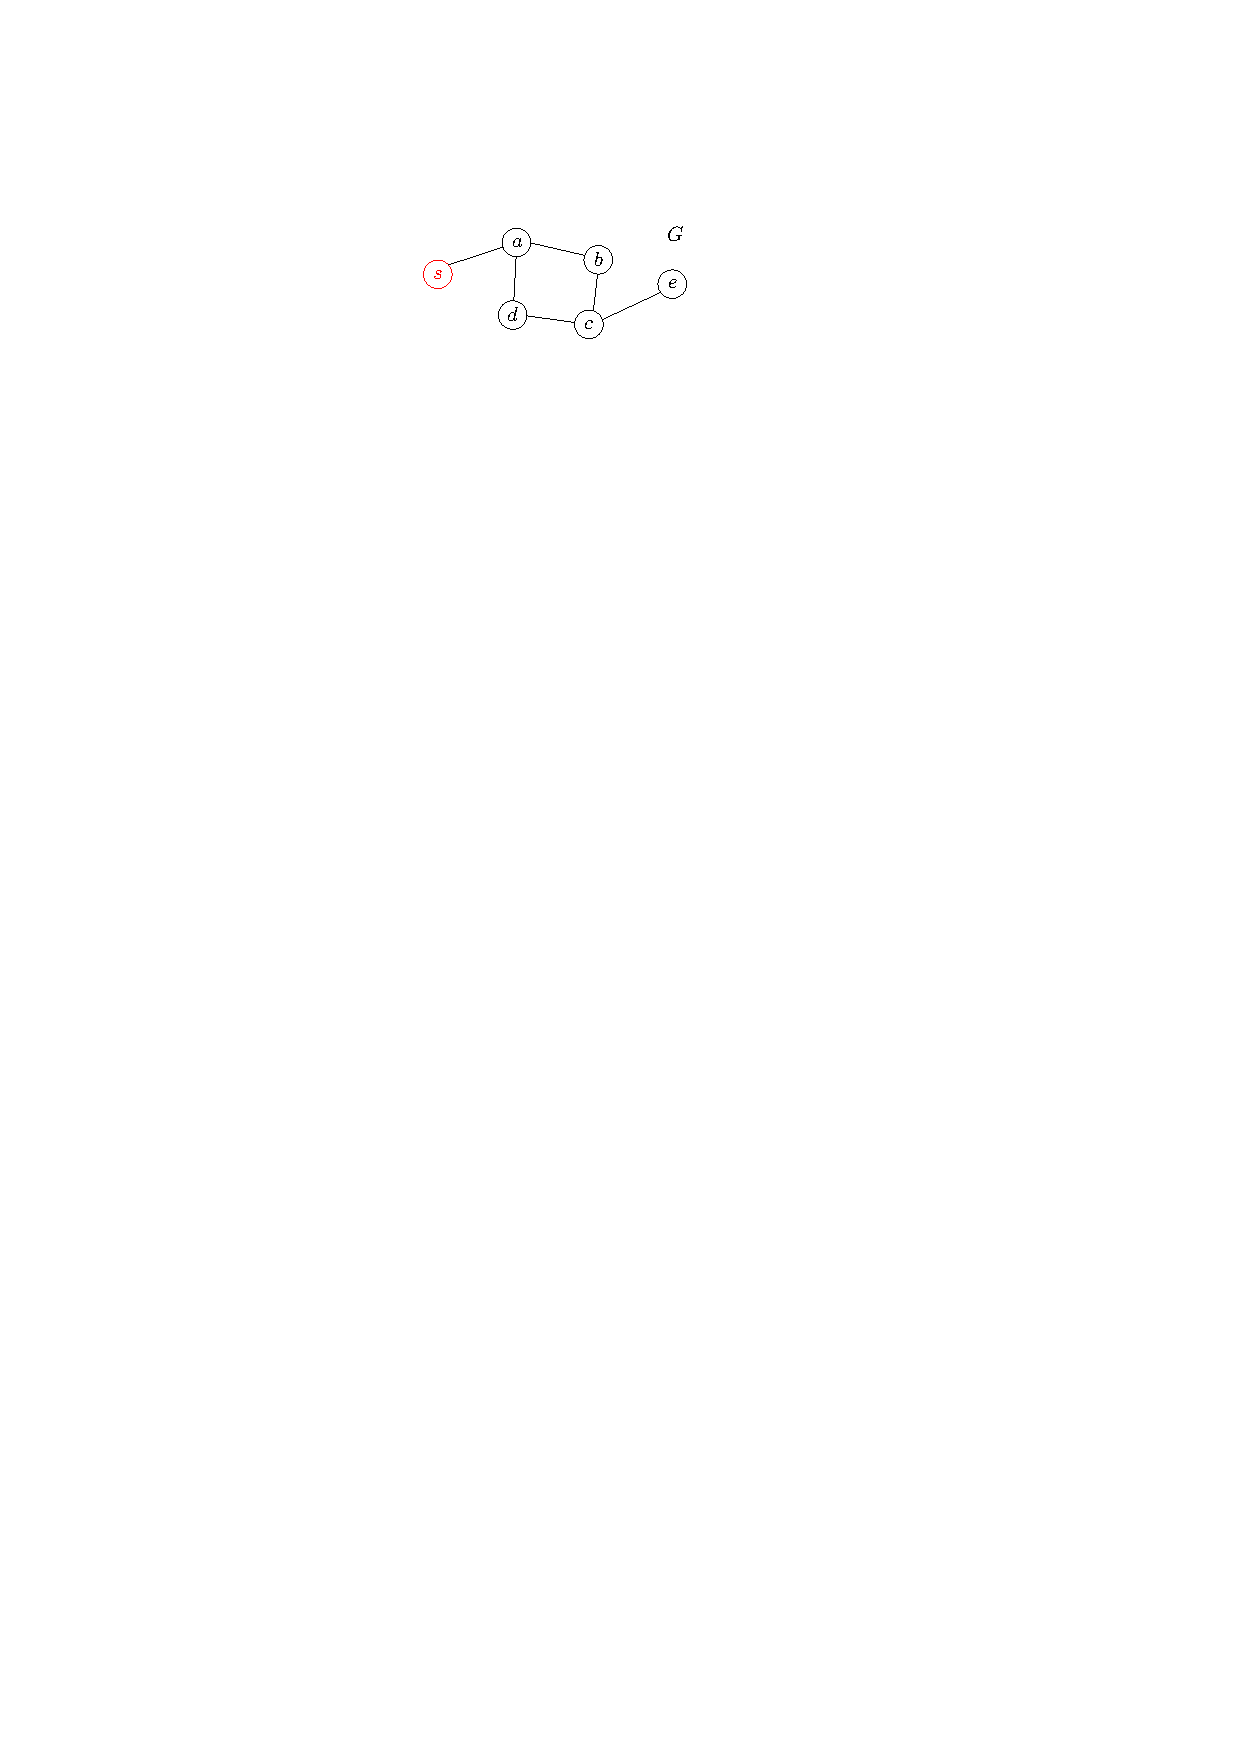
\includegraphics[height=3cm]{fig-graph.pdf}
\end{center}

\begin{solution}
\textbf{Please write down your solution to Problem 2 here.}
\vspace{10pt}\\
We solve the problem by BFS. Consider a BFS tree of the graph, we view $s$ as the root, 
and perform a level-order traversal. For each node, we count the number of it on that level as the number of shortest paths.
For the neighbors of that node, if the number of shortest paths has not been counted for a neighbor, 
we append it to the queue that maintains the BFS tree, otherwise we just ignore it, because it must have been studied in a higher level,
and the node's appearance in the current level does not corresponds to a shortest path.
\vspace{10pt}\\
The pseudocode is as follows:
\vspace{10pt}\\
\begin{lstlisting}[language=Python]
class Node:

    def __init__(self):
        self.neighbors = []

    def add_neighbor(self, other):
        self.neighbors.append(other)
        other.neighbors.append(self)

def COUNT(G, s):

    (V, E) = G 
    # V: list of Node; E: list of tuples of 2 Nodes
    for edge in E:
        edge[0].add_neighbor(edge[1])

    cnt = {}
    queue = [s]
    while queue != []:
        L = len(queue)
        print(L)
        for u in queue[:L]: 
            cnt[u] = cnt.get(u, 0) + 1
            print(u.neighbors)
            for v in u.neighbors:
                if v not in cnt.keys():
                    queue.append(v)
        queue = queue[L:]

    L = [(item[0], item[1]) for item in cnt.items()]
    return L
\end{lstlisting}
This algorithm is correct because it handles the length of path by referring to the depth of the level in the BFS tree.
Because only the shortest path will be considered, each edge will be visited once and only once.
The sum of the number of times each node is visited is $O(m)$, therefore, this algorithm is $O(m)$ (and consequently $O(m+n)$).
\end{solution}

\problem{3: Reaching the one [$15$ pts]}
Let $n \geq 3$ be a given positive integer and we are going to play a game as follows.
During the game, we have a number $k$ which is initially equal to $2$.
In each round of the game, we are allowed to change the current number $k$ to a new number in one of the following ways:
\begin{itemize}
    \item \textbf{Type-A:} Change $k$ to $(k+1) \text{ mod } n$.
    \item \textbf{Type-B:} Change $k$ to a divisor of $k$ that is greater than $1$.
    \item \textbf{Type-C:} Change $k$ to $k^2 \text{ mod } n$.
\end{itemize}

Note that the above three rules guarantee that our number $k$ is always in the range $\{0,1,\dots,n-1\}$ during the entire game.
The game terminates when $k$ becomes $1$.
Our goal is to finish the game in \textit{fewest} rounds.
For example, suppose $n = 91$ and we can play the game as follows.
\begin{itemize}
    \item \textbf{Round 1:} $2 \Longrightarrow 3$ using Type-A change.
    \item \textbf{Round 2:} $3 \Longrightarrow 9$ using Type-C change.    
    \item \textbf{Round 3:} $9 \Longrightarrow 81$ using Type-C change.
    \item \textbf{Round 4:} $81 \Longrightarrow 27$ using Type-B change.
    \item \textbf{Round 5:} $27 \Longrightarrow 1$ using Type-C change.    
\end{itemize}
As you can verify, this is an optimal solution.
Design an algorithm $\textsc{Game}(n)$ which returns an optimal solution to the game as a list.
So $\textsc{Game}(91)$ should return $[2,3,9,81,27,1]$ (or another solution with $5$ rounds).
Describe the basic idea and give the pseudocode.
Briefly justify the correctness and analyze the time complexity.
Your algorithm should run in $O(n \log n)$ time.

(\textbf{Hint:} Formulate the problem as a graph problem with $n$ vertices and $O(n \log n)$ edges.)

\begin{solution}
\textbf{Please write down your solution to Problem 3 here.}
\vspace{10pt}\\
We construct a graph based on the problem setting: all the possible remainders of $n$: $0,1,\dots,n-1$ are constructed as n vertices.
\vspace{10pt}\\
For Type-A operation, we connect vertex $k$ to vertex $k+1$ for $k=0,1,\dots,n-2$, and connect $n-1$ to 0.
\vspace{10pt}\\
For Type-B operation, we connect vertex $k$ to all its divisors larger than 1.
\vspace{10pt}\\
For Type-C operation, we connect vertex $k$ to $k^2$(mod $n$) for $k=2,\dots,n-1$.
\vspace{10pt}\\
Next, we consider the total number of directed edges. For Type-A, the number of directed edges is $n$;
for Type-B, the total number of edges is $\lfloor\frac{n-1}{2}\rfloor+\lfloor\frac{n-1}{3}\rfloor+\dots+\lfloor\frac{n-1}{n-1}\rfloor$;
for Type-C, the total number of edges is $n-2$. 
\vspace{10pt}\\
Therefore, the total number of directed edges $n+\lfloor\frac{n-1}{2}\rfloor+\lfloor\frac{n-1}{3}\rfloor+\dots+\lfloor\frac{n-1}{n-1}\rfloor+n-2
<n+(n-1)\cdot(\frac{1}{2}+\dots+\frac{1}{n-1})+n<n\cdot(1+\frac{1}{2}+\dots+\frac{1}{n})+n$.
By integral test, $\int_{1}^{n}\frac{1}{k}dk<\sum_{k=1}^{n}\frac{1}{k}<\int_{1}^{n}\frac{1}{k}dk+1$, where $\int_{1}^{n}\frac{1}{k}dk=\ln(n)$.
Therefore, $\sum_{k=1}^{n}\frac{1}{k}=O(\log(n))$. Also, $n$ is $O(n\log(n))$, hence the number of directed edges is $O(n\log(n))$.
\vspace{10pt}\\
Next, we perform a BFS search on this graph $G$. We use a queue to maintain the BFS procedure. 
We first append the starting vertex 2 to the queue. 
Every time, for the first vertex in the queue, if it's 1, we quit the BFS; otherwise we append all of its unvisited neighbors to the end of the queue,
and mark the current vertex the previous vertex of all its neighbors (if a neighbor does not have a recorded previous vertex).
\vspace{10pt}\\
This algorithm can always find the shortest path between 2 and 1, because the nearest vertex will always come to the head of the queue.
So when 1 is visited, the path is guaranteed to be shortest. 
\vspace{10pt}\\
The time complexity of this algorithm is $O(n\log(n))$ because the total number of edges in the graph is $O(n\log(n))$,
and each edge is visited at most once.
\vspace{10pt}\\
The pseudocode is given as follows:
\begin{lstlisting}[language=Python]
class Vertex:

    def __init__(self, val):
        self.val = val
        self.neighbors = []

    def add_neighbor(self, other):
        self.neighbors.append(other)

def GAME(n):
    V = [Vertex(i) for i in range(n)]
    # Type A edge
    for i in range(n - 1):
        V[i].add_neighbor(V[i + 1])
    # Type B edge
    for i in range(2, n):
        for j in range(2, i):
            if i % j == 0:
                V[i].add_neighbor(V[j])
    # Type C edge
    for i in range(2, n):
        if i ** 2 % n != i:
            V[i].add_neighbor(V[i ** 2 % n])

    # BFS
    visited = [0 for i in range(n)]
    prev = [-1 for i in range(n)]
    queue = [2]
    while queue != []:
        head = queue[0]
        queue = queue[1:]
        visited[head] = 1
        if head == 1:
            break
        for n in V[head].neighbors:
            if not visited[n.val]:
                queue.append(n.val)
                if prev[n.val] == -1:
                    prev[n.val] = head 

    sol = [1]
    while sol[-1] != -1:
        sol.append(prev[sol[-1]])
    return sol[-2::-1]
\end{lstlisting}
\end{solution}

\problem{4: Finding a strongly connected component [$10$ pts]}
Given a \textit{directed} graph $G = (V,E)$ and a vertex $s \in V$, we want to compute the strongly connected component of $G$ containing $s$.
Design an algorithm $\textsc{SCC}(G,s)$ which returns the set of vertices of $G$ that lie in the same strongly connected component as $s$.
Describe the basic idea and give the pseudocode.
Briefly justify the correctness and analyze the time complexity.
Your algorithm should run in $O(n+m)$ time, where $n = |V|$ and $m = |E|$.

(\textbf{Hint:} By definition, a vertex $v$ is in the same strongly connected component as $s$ iff $v$ is reachable from $s$ and $s$ is reachable from $v$. We already know how to find the vertices reachable from $s$ using DFS. Can you use a similar idea to compute the vertices from which $s$ is reachable?)

\begin{solution}
\textbf{Please write down your solution to Problem 4 here.}
\vspace{10pt}\\
For each node $u$, we store all the nodes $v$ that $(u,v)\in E$ as its \textbf{out-neighbors} and all the nodes $w$ that $(w,u)\in E$ as its \textbf{in-neighbors}.
Then we perform DFS based on out-neighbors to obtain all the nodes that $s$ can reach, and DFS based on in-neighbors to obtain all the nodes that can reach $s$.
Lastly, we take the intersection of the two results, so that we can obtain the set of points in the strongly connected components containing $s$.
\vspace{10pt}\\
This algorithm is correct, as we know DFS can be used to obtain all the nodes that $s$ can reach,
so we can obtain all the nodes that can reach $s$ if we go along the directed edges in reversed direction. 
\vspace{10pt}\\
The time complexity to process in-neighbors and out-neighbors is $O(m)$. The time complexity of DFS is $O(n+m)$. Therefore, the time complexity of the whole algorithm is $O(n+m)$.
\vspace{10pt}\\
The pseudocode is as follows:
\begin{lstlisting}[language=Python]
class Node:

    def __init__(self, val):
        self.val = val
        self.neighbors = [[], []]
        # 0 for in, 1 for out

    def add_neighbor(self, other):
        self.neighbors[1].append(other)
        other.neighbors[0].append(self)
        # add a edge from self to other

def SCC(G, s):

    (V, E) = G
    for (u, v) in E:
        u.add_neighbor(v)
    
    res = [set(), set()]
    # res[0] for all the nodes can be reached from s;
    # res[1] for all the nodes that can reach s
    def DFS(u, direction = 0):
    # direction = 0 for in-neighbors, 1 for out-neighbors
        res[direction].add(u)
        for v in u.neighbors[direction]:
            if v not in res[direction]:
                DFS(v, direction = direction)
    
    DFS(s, 0)
    DFS(s, 1)
    ans = res[0].intersection(res[1])
    ans.remove(s)
    return ans
\end{lstlisting}
\end{solution}

\end{document}